\subsection[Amplitude]{Amplitude: $y_{max}$ o. $s_{max}$ o. $\hat{y}$ o. $\hat{s}$ (Basiseinheit: $m$)}

Die maximale Elongation (=\glqq Auslenkung\grqq) der Schwingung.


\subsection[Periodendauer]{Periodendauer: $T$ (Basiseinheit: $s$)}
	
Die Zeit, die es dauert bis der schwindende Körper an der selben Stelle von der selben Richtung aus angelangt ist. Beispielsweise vom positiven Schwingungsmaximum (\glqq Berg\grqq) zum nächsten oder von der Nullstelle (\glqq Ruhelage\grqq) zur 2. darauffolgenden Nullstelle.

Davon abgeleitet:
\begin{itemize}
	\item Frequenz: $f=\frac{1}{T}$ (Basiseinheit: $Hz=\frac{1}{s}$)
	
	Anzahl der Perioden pro Sekunde.
	\item Winkelgeschwindigkeit: $\omega=2 \pi f=\frac{2 \pi}{T}$ (Basiseinheit: $\frac{rad}{s}$)
		
	Änderung des Winkels über der Zeit, wobei eine ganze Periode mit $360 \degree$ im Grad oder, im Physikunterricht verwendet, mit $2 \pi$ im Bogenmaß (eng: \glqq Radian\grqq) bezeichnet wird.\footnote{Umrechnung des Winkels $\alpha$ von Grad nach Bogenmaß: $\alpha_{rad} = \alpha_{deg} \cdot \frac{2\pi}{360 \degree} = \alpha_{deg} \cdot \frac{\pi}{180 \degree} $}
\end{itemize}


\subsection[Phasenverschiebung]{Phasenverschiebung: $\phi$ (Basiseinheit: $rad$)}
	
Wenn sich der Schwingungskörper zum Startzeitpunkt $t=0$ nicht in der Ruhelage $y=0$ befindet muss die Phasenverschiebung, z.B. zur Aufstellung der Schwingungsgleichung (\referenz{subsec:schwingungsgleichungen}), berücksichtigt werden. Die Phasenverschiebung gibt den Abstand von der y-Achse zum nächsten Durchlauf der Ruhelage von der negativen Seite.

	\begin{wrapfigure}{r}{0.5\textwidth} \label{phasenverschiebung}
	
		\vspace{-10pt}
		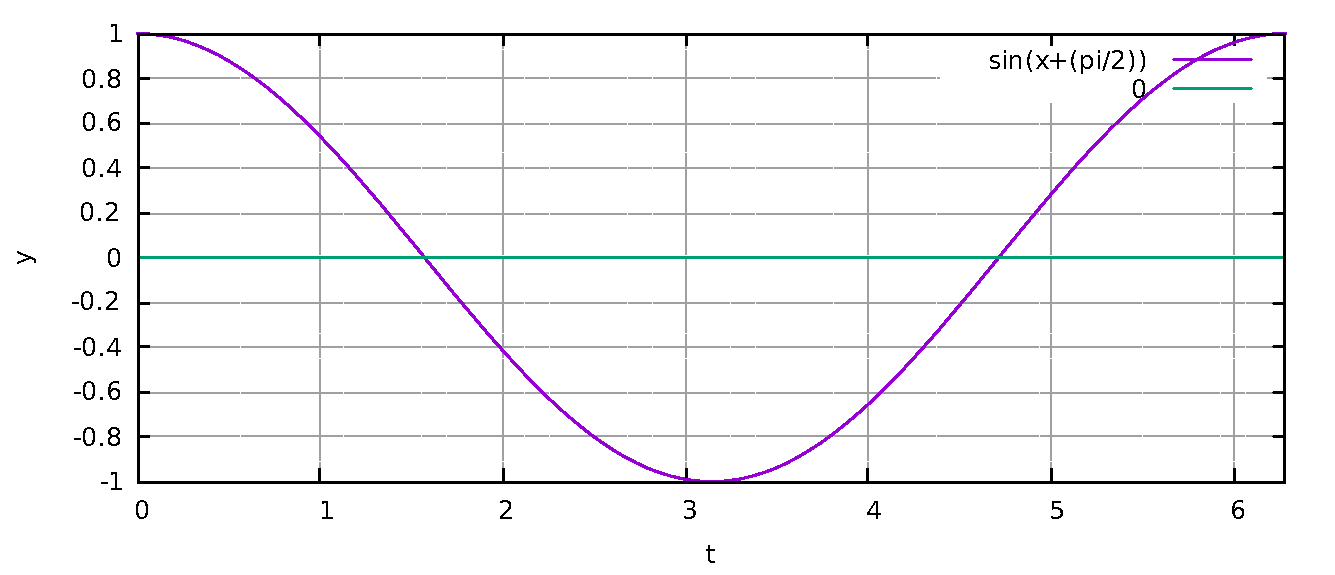
\includegraphics[width=0.48\textwidth]{phasenverschiebung}
		\vspace{-13pt}
		\caption{Phasenverschiebung um $+\frac{3\pi}{2}$}
		\vspace{-5pt}
	
	\end{wrapfigure}

Im nebenstehenden Diagramm beträgt die Phasenverschiebung $\phi = +\frac{3\pi}{2}$, also ein Drei-Viertel der Periode. Man könnte ebenfalls sagen, die Phasenverschiebung beträgt $\phi = -\frac{\pi}{2}$, also minus Ein-Viertel der Periode. Beides ist äquivalent, jedoch ist es leichter mit einer positiven Phasenverschiebung zu rechnen.
	